\section{Системное проектирование}
\label{sec:domain}

В данном разделе будет произведён обзор предметной области задачи, решаемой в рамках дипломного проекта; рассмотрен вопрос об архитектуре разработанного программного обеспечения.
Также будут рассмотрены принципы работы структурных блоков, реализованных в программном обеспечении, разработанном в рамках дипломного проекта.

\subsection{Анализ предметной области}
\label{sub:domain:bayes_net}

Как уже упоминалось выше, целью настоящего дипломного проекта является создание сервиса и клиентского приложения к нему, предоставляющего возможность хранить и редактировать различные пользовательские данные, предотвращая их утечку третьим лицам, скрывая их сигнатуру.

Клиентское приложение взаимодействует с сервером, посредством API. Сервис по взаимодействию с базой данных поставляется вместе с драйвером СУБД и инкапсулирует всю логику. Клиент должен предоставлять интерфейс, с помощью которого пользователь сможет получать и сохранять информацию, предоставляемую сервисом.

Важным моментом при разработке приложения является то, что система является много"=компонентной. К разным компонентам системы может применяться различные архитектурные подходы.

Серверная часть приложения содержит монолитное крипто"=графическое ядро. В первую очередь это обусловлено в простоте реализации. Его недостатком может быть большой набор требований к функциональности приложения, в результате чего будет затруднена поддержка и расширяемость. При добавлении нового функционала программа будет масштабироваться, требуя больше времени и ресурсов на поддержку.
Подобный архитектурный прием в системах со слабо связанной архитектурой, каждый компонент которой обладает минимальными знаниями о других компонентах, позволяет использовать стороннее программное обеспечение. Такая практика позволит во много раз сократить расходы на разработку программного продукта.

Для обеспечения приложения способностью масштабироваться при разработке других слоев, вне ядра, использовался модульный подход к разработке программного обеспечения, основанный на использовании распределённых, слабо связанных, заменяемых компонентов, оснащённых стандартизированными интерфейсами для взаимодействия по стандартизированным протоколам SOA~\cite[с.~16\,--\,17]{sicp_2006_ru}, структура которого изображена на рисунке~\ref{fig:domain:bayes_net}.

\begin{figure}[ht]
\centering
  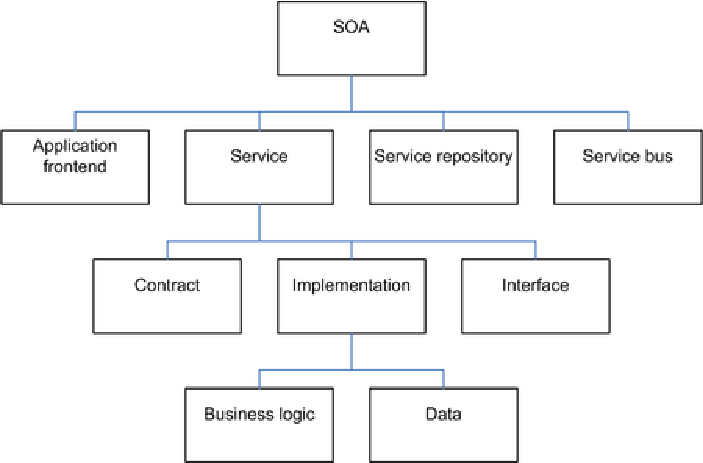
\includegraphics[scale=1]{soa_struct.pdf}
  \caption{ Структура протокола SOA. }
  \label{fig:domain:bayes_net}
\end{figure}

Программные комплексы, разработанные в соответствии с \foreignlanguage{english}{SOA} были реализованы как набор веб-служб, взаимодействующих по протоколу \foreignlanguage{english}{SOAP}. Интерфейсы компонентов в сервис-ориентированной архитектуре инкапсулируют детали реализации от остальных компонентов, таким образом, обеспечивая комбинирование и многократное использование компонентов для построения сложных распределённых программных комплексов, обеспечивая независимость от используемых платформ и инструментов разработки, способствуя масштабируемости и управляемости создаваемой системы.

Управление информацией между клиентским и серверным приложением осуществляется по REST протоколу. REST сервис полностью основывается на протоколе передачи данных. Для HTTP действие над данными задается с помощью методов: GET, PUT, POST, DELETE. Таким образом, действия CRUD могут выполняться как со всеми четырьмя методами, так и только с помощью GET и POST запросов~\cite{restfull}.

Основные возможности разработанного одностраничного приложения заключаются в написании одного сервиса по выдаче модели отображения и множества сервисов для взаимодействия пользователя с базой данных. Такие возможности заключаются в следующем:
\begin{enumerate}
  \item Пользователь получает возможность создавать личное хранилище, обладает уникальным идентификатором, который проверяется каждый раз, когда он совершает действия изменяющие состояние сервиса. Если конкретный пользователь пытается просмотреть записи хранилища, которое находится на в шифрованным виде, либо запись, которая принадлежит хранилищу доступного локально, его идентификатор поддается дешифровке и проверяется на валидность в рамках всего цикла жизни клиента.
  \item Пользователь может просматривать и редактировать определенные группы данных в хранилищах, дешифрованных его публичным ключом на клиенте, полученным при аутентификации.
  \item Пользователю предоставляется возможность добавлять, удалять и редактировать новые поля и хранилища.
  \item При редактировании записей, данные шифруются публичным ключом и отправляются на сервер, где подвергаются дешифровке приватным ключом и вторичному шифрованию синхронным методом.
\end{enumerate}

\subsection{Идентификация объектов предметной области}
\label{sub:domain:object}

В разрабатываемом приложении можно выделить четыре слоя, связанных между собой различными уровнями обструкции. И хотя у них есть общие части, такие, как модель данных, они вполне могут разрабатываться независимо друг от друга:
\begin{itemize}
  \item Client Layer;
  \item Application Server Layer;
  \item Business Layer;
  \item Data Layer.
\end{itemize}

Эта модель объединяет два основных слоя: Client Layer и \foreignlanguage{english}{Application Server Layer}. Таким образом, структура программы напоминает классическую трехуровневую модель~\cite[с.~308\,--\,401]{sicp_2006_ru}, в которой имеется три явно выраженных слоя. Пользовательский интерфейс, реализованный в Client Layer и \foreignlanguage{english}{Application Server Layer}, представляет собой блок отображения данных. Data Layer приложения, управляемый Business Layer, представляет собой уровень доступа к базе данных. Сюда относятся сервисы, которые поставляются драйвером СУБД, классы-посредники, и синглтоны. База данных представляет уровень Data, самый нижний уровень в иерархии.

Каждый из слоев имеет свой уровень абстракции, согласно которому каждый слой не знает о реализации другого. Все блоки работают по принципу черного ящика, каждому из которых необходимо лишь знать о входных и выходных параметрах. На основании этого можно более детально разобрать каждый элемент системы на подсистемы, поясняющие общий принцип взаимодействия модулей на разных слоях взаимодействия.

Business Layer представляет слой обработки пользовательских данных и событий Data Layer, обеспечивает высокоуровневый интерфейс для \foreignlanguage{english}{Application Server Layer}, скрывая реализацию Data Layer. Текущий слой обеспечивает связывание модулей, решает проблему связывания подписчиков и издателей путем автоматической регистрации событий, который автоматически вызывает нужные привязки на основе соглашения об именовании.
Существование Business Layer подразумевает регистрацию всех компонентов, которые могут подписываться на события, регистрацию всех событий на которые можно подписаться и набор событий компонентов.

Приемущество разработанной архитектуры связано с отсутствием зависимости между компонентами приложения. Это дает основание для формирования свободной иерархии пакетов, представляя возможность использовать разработанное приложение при построении более сложной архитектуры в качестве стороннего компонента или ядра. Кроме того, благодаря низкому уровню связанности кода, отдельные модули можно также использовать повторно в сторонних продуктах.

\subsection{Декомпозиция объектов предметной области}
\label{sub:domain:object_decomp}

На каждый логически выделенный слой программы возлагаются определенные задачи, решение которых делегируется сущностям более низкого порядка детализации. Кроме того, каждый блок программы так или иначе связан с остальными блоками, чтобы обеспечить работоспособность всего приложения в целом. Связь, как правило, реализуется посредством обмена данными утвержденной сигнатуры между блоками.

Блок пользовательского интерфейса представляет собой множество пользовательских компонентов, взаимодействующими между всеми остальными блоками программы. Он отвечает за отрисовку страницы в браузере. Основной его функцией является представление того или иного компонента пользователю по запросу от блока контроля и обработки событий. При этом он может обеспечивать рендеринг страницы из разных источников в рамках политики общего происхождения.

Блок контроля и обработки событий определяет наличие изменений состояния блоков пользовательского интерфейса и формирования запросов на сервер, производит оповещение подписчиков о текущем состоянии, служебных сообщениях, не относящиеся напрямую к работе текущего модулю. В первую очередь, это сообщения соединения с сервером, истечение срока действия авторизационный данных, системные ошибки во время исполнения процедур. Блок не имеет представления, как устроено отображение модели, и как работают сервисы, направленные на обновление модели. Блок контроля и обработки событий связан напрямую с блоком пользовательского интерфейса. Все действия и события, происходящие на странице, так или иначе обращаются к контроллеру. Контроллер, после обработки сервисом, возвращает обработанную модель событию на клиентской части, где происходит изменение отображения страницы.

Блок криптографической защиты данных представляет собой совокупность средств и методов шифрования/дешифрования различных типов данных, проверки электронной подписи и сбор данных для их дальнейшей обработки.

Блок формирования запросов на сервер осуществляет имплементацию данных и их валидацию, а также формирование запросов к серверу соблюдая их иерархию. Все данные, которые отправляются с клиентской части на серверную, проходят проверку в текущем блоке. При соответствии сигнатуры, объекты данных передаются далее на сервер. Все правила, которым должна соответствовать модель, задаются на этапе разработки модели страницы и блоков валидации данных.

Блок серверной обработки HTTP-запросов представляет собой систему маршрутизации по принципу REST архитектуры. Основной причиной для ее внедрении послужило то, что большое количество логики на клиенте необходимо структурировать. К тому же в перспективе решение может масштабироваться. В этом случае возможно появление специальной клиентской части с ограниченным функционалом в качестве мобильного приложения. Не исключено появление и десктопных клиентов приложения. Приложение в основном использует JSON\footnote{\url{http://www.w3schools.com/json/}} для передачи информации и загрузки ее с сервера. Необходимость в максимальной расширяемости системы подразумевает, что к одной и той же точке API сервера могут подключаться разные версии приложения.

Блок обработки пользовательских событий на серверной стороне осуществляет проверку идентификационных данных пользователя, обеспечивая целостность и защиту от фальсификации передаваемой информации. Он может быть использован для обнаружения несанкционированных изменений данных, как преднамеренных, так и случайных, во время жизненного цикла приложения. Любая несанкционированная попытка получить доступ к данным посредствам неавторизованного подключения будет отклонена, а блок известит клиент о попытке несанкционированного доступа.

Блок базы данных представляет собой хранилище всей информации, с которой может работать приложение и пользователь. Блок реализует асинхронную репликацию в конфигурации, основанную на передаче журнала изменений с ведущего узла на ведомые, тем самым поддерживается автоматическое восстановление в случае выхода из строя ведущего узла. Принимает параметры, делает выборку или обновление записей в базе, согласно определенному сценарию, и возвращает набор данных, либо результат выполнения сервису приложения.

Блок объектной модели базы данных и блок обеспечения доступа к базе данных предоставляются драйвером СУБД на уровне платформы. Оба сервиса работают по принципу «черного ящика» – на вход передаются параметры, на выходе возвращаются данные.